\documentclass[notes=show,handout]{beamer}
\usepackage{amsmath}
\usepackage{graphicx}
\usepackage{mathpazo}
\usepackage{hyperref}
\usepackage{multimedia}
\usepackage{epstopdf}
\usepackage{tikz}
\usetikzlibrary{shapes,backgrounds}

\setcounter{MaxMatrixCols}{10}
\usetheme{Madrid}
\newtheorem{conj}{Conjecture}[section]
\newtheorem{aim}{Aim}[section]

\newtheorem{remark}{Remark}[section]
\newtheorem{proposition}{Proposition}[section]
\newtheorem{interpretation}{Interpretation}[section]
\newtheorem{goal}{Goal}[section]
\newtheorem{statement}{Statement}[section]
\newtheorem{aes}{Aim \& Scope}[section]



\newcommand{\mbf}[1]{\mathbf{#1}}
\newcommand{\beq}{\begin{equation}}
\newcommand{\eeq}{\end{equation}}
\newcommand{\bea}{\begin{eqnarray}}
\newcommand{\eea}{\end{eqnarray}}
\newcommand{\ba}{\begin{array}}
\newcommand{\ea}{\end{array}}
\newcommand{\bi}{\begin{itemize}}
\newcommand{\ei}{\end{itemize}}
\newcommand{\ben}{\begin{enumerate}}
\newcommand{\een}{\end{enumerate}}
\newcommand{\nn}{\nonumber}
\newcommand{\fn}[1]{\footnote{#1}}
\renewcommand{\r}{\right}
\renewcommand{\l}{\left}
\long\def\symbolfootnote[#1]#2{\begingroup\def\thefootnote{\fnsymbol{footnote}}\footnote[#1]{#2}\endgroup}


\usepackage{color}
\newcommand{\hilight}[1]{\colorbox{yellow}{#1}}

\begin{document}

\title[S110015]{Probability 1}
\subtitle{A reminder of Mathematics}
\author[Flores Agreda]{Daniel {Flores Agreda}}
% \author[La Vecchia]{Davide La Vecchia}
\date{Spring Semester 2021}
\maketitle



% \begin{frame}
% \frametitle{Preliminaries}
%
% \color{red}Ê\textbf{Time frame:} \color{black}
%
% \vspace{0.2cm}
%
% \begin{itemize}
% \item Lectures (no recording): Thur. from 12 to 14 (MR280) \vspace{0.5cm}
%
% \item Exercises (no recording, text \& solutions available on Chamilo):  Thur. from 16 to 18 (MS130)
%
% \end{itemize}
%
% \vspace{0.85cm}
%
% \color{red}Ê\textbf{Exam:} \color{black} Written exam \textbf{open-book, 2 hrs}
%
% \vspace{0.85cm}
%
% \color{red}Ê\textbf{Book:} \color{black} \textit{A first course in probability}, S. Ross (any edition), Ed: Pearson New International Edition. This is the main reference book for the whole course.
%
%
% \end{frame}



% \begin{frame}
% \frametitle{Preliminaries}
% Let us start by a general statement:
%
% \vspace{0.35cm}
% \begin{statement}
% Probability is defined as the measure of the ``likelihood'' of an event or random outcome. \\
% \end{statement}
%
%
% \vspace{0.35cm}
%
% Another way of saying that is: \\ \vspace{0.25cm}
%
% \begin{center}
% \color{red}\textbf{Q.}: ``What is the chance of something happening?'' \color{black}
% \end{center}
%
% \vspace{0.35cm}
%
%
% To answer this question we make use of Probability. Indeed, Probability is all about the certainty/uncertainty and the prediction of something
% happening. Some events are impossible, other events are certain to occur, while many are possible, but not certain to occur...
%
% \end{frame}

% \begin{frame}
% \frametitle{Preliminaries}
%
%
% \vspace{1.25cm}
%
% \begin{quote}
%  {\Large `In this world there is nothing certain but death and taxes.'}\\
% \end{quote}
%
% \vspace{1.25cm}
% \vspace{2.25cm}
%
% \begin{flushright}
% {Benjamin Franklin}
% \end{flushright}
%
% %\vspace{2.25cm}
%
%
% \end{frame}


% \begin{frame}
% \frametitle{Preliminaries}
%
%
% \begin{figure}[h!]
% \centering
% 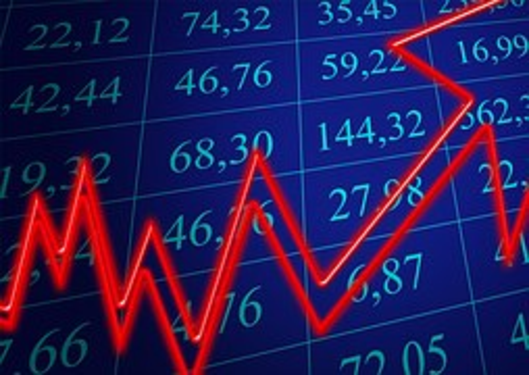
\includegraphics[width=0.4\textwidth,height=0.5\textheight]{profit.pdf}
% \end{figure}
%
%
% \begin{figure}[h!]
% \begin{flushright}
% 
\includegraphics[width=0.3\textwidth,height=0.3\textheight]{tipoS.pdf}
% \end{flushright}
% \end{figure}
%
%
%
% \end{frame}
%
%
%
% \begin{frame}
% \frametitle{Preliminaries}
%
% \begin{example} [Stock price evolution]
% Let us imagine that we are going to model the  \textbf{uncertainty} characterizing the Stock price of an asset by a simple model. With probability $p=1/2$
% the stock price moves up of a factor $u$, and with probability $1-p$ the price moves down of a factor $d$. We denote the price at time $t_1$  by $u S_0 $ if the price goes up, and by $d S_0 $  if the price goes down. \\ \vspace{1cm}
%
% Let us set $S_0=1$, $u=2$ and $d=1/2$. Can we say something about the price at time $t_2$?
% \end{example}
%
% \end{frame}
%
% \begin{frame}
% \frametitle{Preliminaries}
%
% \begin{example} [cont'd]
% \begin{small}
%  The price evolution is represented by a tree:
% \tikzstyle{bag} = [text width=8em, text centered]
% \tikzstyle{end} = []
% \begin{tikzpicture}[sloped]
%    \node (a) at ( 0,0) [bag] {$\$ 1$};
%    \node (b) at ( 4,-1.5) [bag] {$\$ d =\$ 0.5$};
%    \node (c) at ( 4,1.5) [bag] {$\$ u= \$ 2$};
%    \node (d) at ( 8,-3) [bag] {$\$ d^2= \$ 0.25$};
%    \node (e) at ( 8,0) [bag] {$\$ ud= \$ du = \$ 1$};
%    \node (f) at ( 8,3) [bag] {$\$ u^2=\$ 4$};
%    \draw [->] (a) to node [below] {$(1-p)$} (b);
%    \draw [->] (a) to node [above] {$p$} (c);
%    \draw [->] (c) to node [below] {$p^2$} (f);
%    \draw [->] (c) to node [above] {$(1-p)p$} (e);
%    \draw [->] (b) to node [below] {$(1-p)p$} (e);
%    \draw [->] (b) to node [above] {$(1-p)^2$} (d);
% \end{tikzpicture}
% \end{small}
% \end{example}
% \end{frame}
%
%
% \begin{frame}
% \frametitle{Preliminaries}
%
%
% \begin{figure}[h!]
% \centering
% 
\includegraphics[width=0.3\textwidth,height=0.2\textheight]{Quantum.pdf}
% \end{figure}
%
%
% \begin{figure}[h!]
% 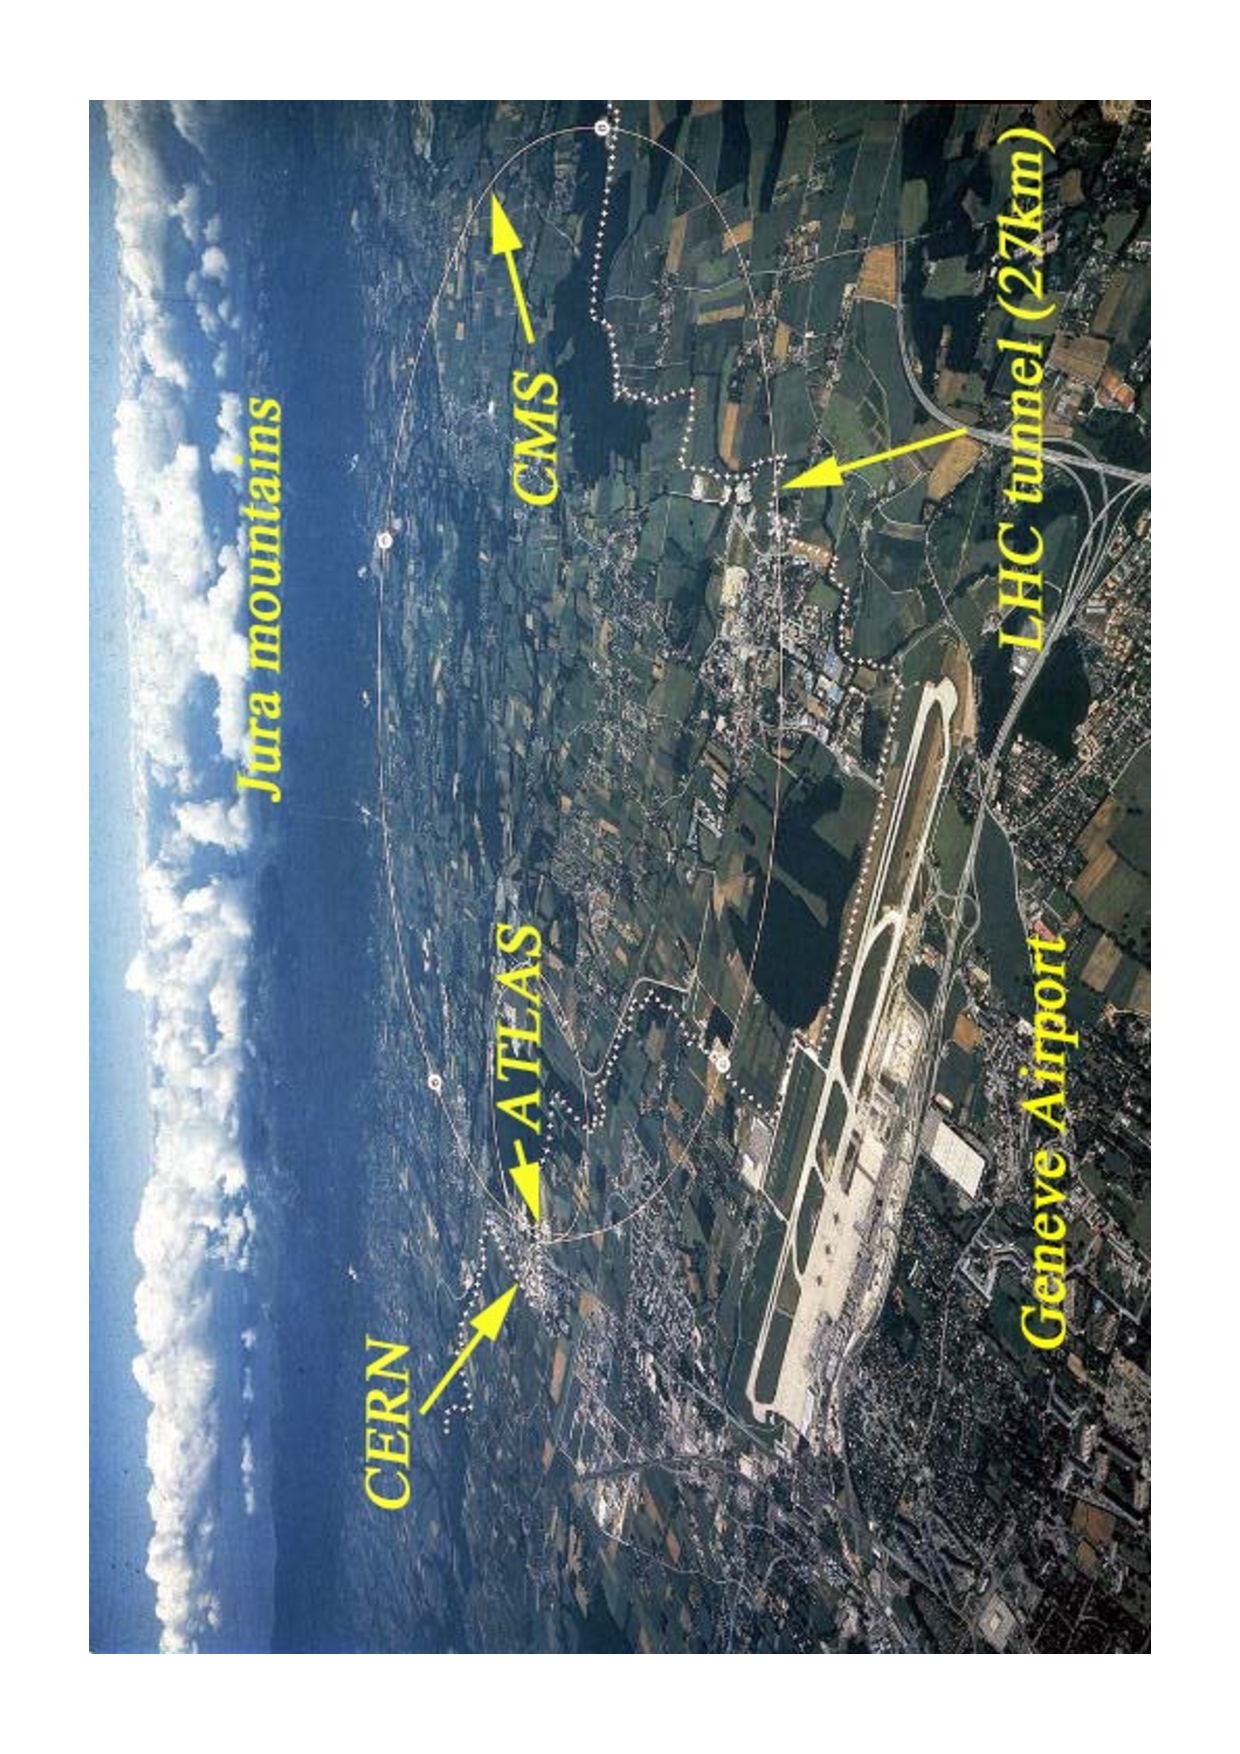
\includegraphics[width=0.4\textwidth,height=0.9\textheight, angle = -90]{cern.pdf}
% \end{figure}
%
%
% \end{frame}
%
% \begin{frame}
% \frametitle{Preliminaries}
%
% \begin{example} [Quanta]
%
% Probability models are the basis for quantum physics: they characterize the \textbf{uncertainty} of properties of single energy ``quanta'' emitted by a ``perfect radiator" with a given temperature ($T$). Specifically, recall the famous Einstein's equation $$\boxed{\mathcal{E} = m c^2}$$ which expresses the energy $\mathcal{E}$  in terms of the mass \underline{$m$, a random quantity,} and $c$, the speed of light. Moreover, consider the geometric energy mean defined by ${\mathcal{E}_G} = c_0 k_B T$, where $c_0 \approx 2.134$ and $k_B$ is Boltzmann's constant. Thus, one can define the random quantity
% $$
% W = \frac{\mathcal{E}}{{\mathcal{E}_G}},
% $$
% which is called \textit{quantum mass ratio}.
%
% \end{example}
% \end{frame}
%
%
%
% \begin{frame}
% \frametitle{Preliminaries}
%
% \begin{example} [cont'd]
% The random behaviour of $W$ can be described by a probability density function:
% \begin{figure}[h!]
% 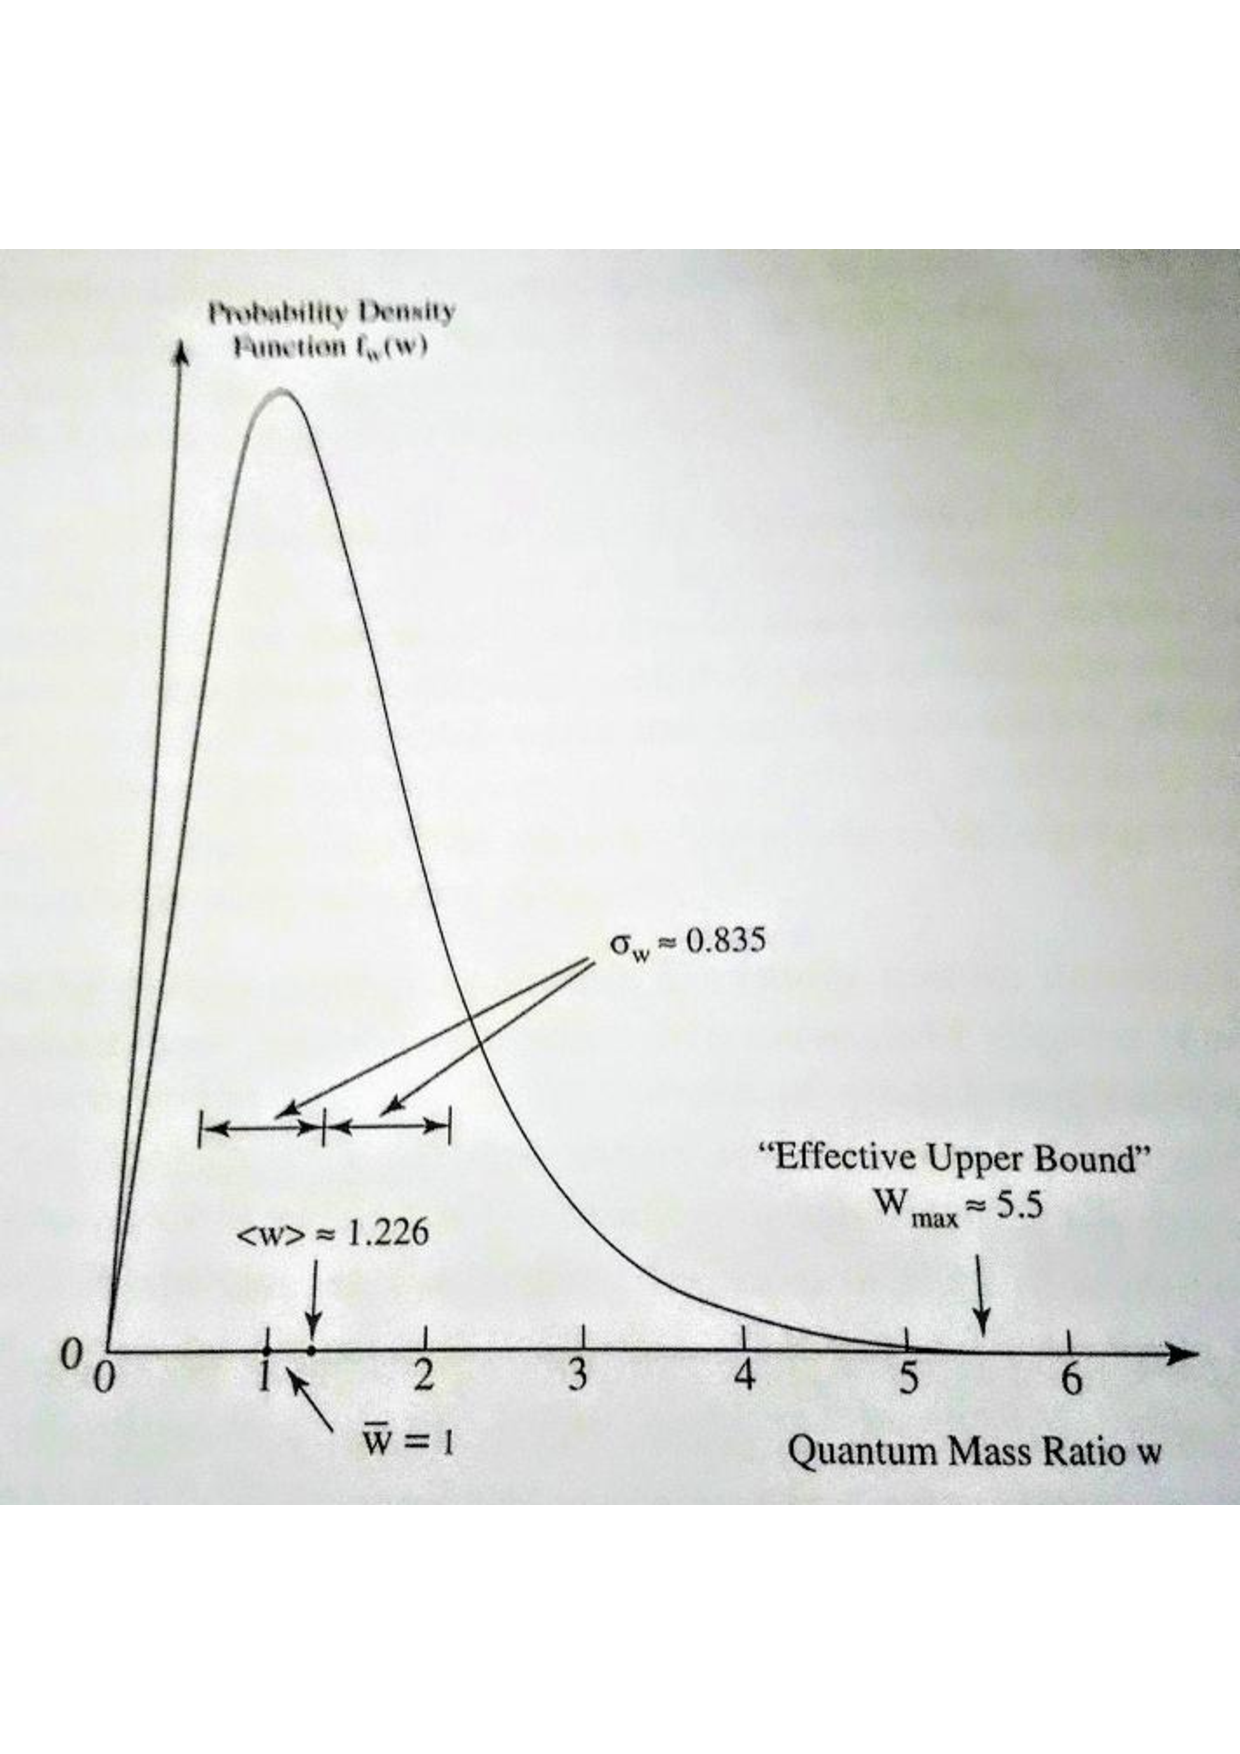
\includegraphics[width=0.4\textwidth,height=0.6\textheight, angle = 0]{W.pdf}
% \end{figure}
%
% \end{example}
% \end{frame}
%
%
% \begin{frame}
% \frametitle{Preliminaries}
%
% In this course, we study \color{blue} Probability \color{black} as a way to introduce \color{blue} Statistics\color{black}. \\
%
% \vspace{0.5cm}
%
% Thus, we do not study Probability as a subject of interest in itself: we do not develop deep probability theory via measure theoretic arguments,
% rather we set up a few principles and methods which will be helpful for Statistics.
%
% \end{frame}
%
%
%
% \begin{frame}
% \frametitle{Preliminaries}
%
% \begin{figure}[h!]
% \centering
% 
\includegraphics[width=0.6\textwidth,height=0.7\textheight]{y.pdf}
% \end{figure}
%
%
%
%
% \end{frame}
%
%
%
%
% \begin{frame}
% \frametitle{Preliminaries}
%
% \color{red} \textbf{Q.} Why is it important to study Probability/Statistics? \color{black}\\
% \vspace{0.5cm}
%
% To understand why we must study Probability/Statistics, it is useful to first understand the answer to the following questions:
% \vspace{0.5cm}
%
% \color{red}\textbf{Q.} What is Statistics? What is Probability? \color{black}
% \vspace{0.5cm}
%
% \textbf{A.} \color{blue} STATISTICS \color{black} deals with the collection, presentation, analysis and interpretation of data in order to make rational decisions. Since, there is uncertainty in the data, we need \color{blue} PROBABILITY\color{black}, which deals with uncertainty.
%
% \end{frame}
%
% \begin{frame}
% \frametitle{Preliminaries}
%
% \begin{aes}
%
% One makes use of Probability to develop methods to deal with uncertainty. Then, one applies these methods in tandem with Statistics to take  decisions under uncertainty.
% \end{aes}
%
% \bigskip
%
% $\leadsto$ Uncertainty is measured in units of \textit{probability},
% which \textit{is the currency of statistics}.
%
% \bigskip
%
% % \item[--]
%
% $\leadsto$ Statistics is concerned with % the \highlighttext{study of uncertainty} and with
% the \textit{study of data}--\textit{driven decision making in the face of uncertainty}.
%
% \end{frame}



%
%\begin{frame}
%\frametitle{Preliminaries}
%
%
%A bit more precisely, \textbf{Statistics}
%
%\vspace{0.2cm}
%
%$\leadsto$  is the science of {`learning
%  from data'} (or of {making sense out of data}), and of
% {measuring, controlling and communicating uncertainty}.
%
%%% \begin{itemize}
%%% \item[--] Statistics can be defined as the science of \present{`learning
%%%   from data'} (or of \highlighttext{making sense out of data}), and of
%%%  \highlighttext{measuring, controlling and communicating uncertainty}.
%
%\medskip
%
%$\leadsto$ is a \textbf{{process}} that includes everything from planning for the collection of data
% and subsequent data management to end-of-the-line activities
% such as drawing conclusions of %numerical facts called
% data and
% presentation of results.
%
%\bigskip
%
%%% \item[--]
%
%
%\end{frame}

\begin{frame}
\frametitle{Overview}

\begin{enumerate}
\item[1.]  Introduction: some fundamental math tools
\item[2.] Basic calculus for probability
\begin{itemize}
\item[-] Random variables
\item[-] Trees
\item[-] Venn diagram
\item[-] Conditional probability
\item[-] Independence \& Bayes' theorem
\item[-] ...
\end{itemize}

\item[3.] Discrete random variables
\begin{itemize}
\item[-] Definitions
\item[-] Expected value and variance
\item[-] Binomial
\item[-] Poisson
\item[-] Negative binomial and hypergeometric
\end{itemize}

\end{enumerate}
\end{frame}


\begin{frame}
\frametitle{Overview}

\begin{enumerate}
\item[4.]  Continuous random variables

\begin{itemize}
\item[-] Definitions
\item[-] Expected value and variance
\item[-] Cumulative distribution function (cdf) and Probability density function (pdf)
\item[-] Some important examples: Uniform, Exponential, Gamma, Normal, logNormal, Student's...
\item[-] Relationships
\end{itemize}

\item[5.] Bivariate random variables

\item[6.] Limit theorems: Weak Law of Large Numbers (WLLN) and Central Limit Theorem (CLT)

\item[7.] Elements of simulations:  numerical methods for the simulation of random variable with a given CDF...

\end{enumerate}

\end{frame}





\begin{frame}
\frametitle{Some mathematical formulas}

To go thought this program, we need math.

\vspace{0.4cm}

For instance, we are going to make use of the following \textbf{powers and logs}:
\vspace{0.4cm}
\begin{itemize}
\item $a^m \cdot a^n = a^{m+n}$;
\item $(a^n)^m = a^{m \cdot n}$;
%\item $\ln(\exp^{a}) = a$;
\item $a=\ln(\exp^{a}) = \ln(e^a)$;
\item $\ln(a^n) = n \cdot \ln a$;
\item $\ln (a \cdot b) = \ln (a) + \ln (b)$;

\end{itemize}

\end{frame}




\begin{frame}
\frametitle{Some mathematical formulas (cont'd)}

The \textbf{derivatives} will also play a pivotal role. For instance:

\bea
 \frac{d x^n}{dx} = n \cdot x^{n-1}, \quad \frac{d \exp^{x}}{dx} = \exp^{x} , \quad
\frac{d \ln({x})}{dx} = \frac{1}{x}, \nn
\eea
and we will make use of some fundamental rules, like e.g.

\begin{itemize}
\item Product rule:
\bea
\frac{d [f(x)\cdot g(x)]}{dx} &=& \frac{df(x)}{dx} g(x) + \frac{dg(x)}{dx} f(x) \nn \\
&=& f'(x) g(x)+ f(x) g'(x) \nn ;
\eea
\item Chain rule: $$ \frac{d f[g(x)]}{dx} =  (f\circ g)'(x) = f'[g(x)] \cdot g'(x). $$
\end{itemize}
\end{frame}


\begin{frame}
\frametitle{Some mathematical formulas (cont'd)}

The \textbf{integrals} will be crucial in many tasks. For instance, recall that:

\begin{itemize}
\item \bea
\int_{a}^{b} \left[c \cdot f(x) + d \cdot g(x) \right]dx = c  \cdot \int_{a}^{b}   f(x) dx + d \cdot \int_{a}^{b}   g(x) dx; \nn
\eea
%\item  A special case of Leibnitz's rule: $$ \frac{d}{dx} \int_{-\infty}^{x} f(s) ds = f(x);$$
%\item
%\bea
%\int_{a}^{b} f(x) dx = \int_{a}^{m} f(x) dx + \int_{m}^{b}  f(x) dx,  \quad { \text{\ for \ } m \in [a,b]; }\nn
%\eea
\item If $f(x) \geq 0, \forall x \in \mathbb{R}$, then
$$ \int_{\mathbb{R}} f(x) dx \geq 0. $$
\item For a continuous function $f(x)$, the indefinite integral is
$$
\int f(x) dx = F(x) + \text{const}
$$
while the definite integral is
$$
F(b)-F(a)= \int_{a}^{b} f(x) dx, \quad b \geq a.
$$
\end{itemize}
\end{frame}


\begin{frame}
\frametitle{Some mathematical formulas (cont'd)}

Besides integrals we are also going to use \textbf{sums}:

\begin{itemize}
\item $$\sum_{i=1}^{n} X_{i} = X_1 + X_2 +....+ X_n,$$
\item For every $\alpha_i \in \mathbb{R}$,  $$\sum_{i=1}^{n} \alpha_i X_{i} = \alpha_1 X_1 + \alpha_2 X_2 +....+ \alpha_n X_n;$$
%whose special case is
%$
%\sum_{i=1}^{n} \alpha X_{i} = \alpha X_{i} = \alpha X_1 + \alpha X_2 +....+ \alpha X_n = \alpha \sum_{i=1}^{n} X_{i}
%$
\item Double sum: a sum with two indices. For instance,
\begin{small}
\bea
\sum_{i=1}^{n} \sum_{j=1}^{m}  x_{i}y_{j}  &=& x_1y_1 + x_1 y_2 +... +x_2y_1+ x_2y_2 +... \nonumber \\
&=& \left(\sum_{i=1}^{n} x_i\right) y_1 +  \left(\sum_{i=1}^{n} x_i\right) y_2 + ... +  \left(\sum_{i=1}^{n} x_i\right) y_m  \nonumber \\
&=& \sum_{i=1}^{n} x_i \sum_{j=1}^{m} y_j. \nonumber
\eea
\end{small}
\end{itemize}
\end{frame}


\begin{frame}
\frametitle{Some mathematical formulas (cont'd)}

Finally, we also rely on some \textbf{combinatorial formulas}. Specifically,

\begin{itemize}
\item Factorial
$$
n! = n \cdot (n-1) \cdot (n-2) \cdot ... \cdot 1;
$$
where $0! =1$, by definition;
\item Binomial coefficient, for $n \geq k$
$$
\binom n k =\frac{n!}{k!(n-k)!} \color{gray}{=C^{k}_n}\color{black}
$$
which is helpful to express the \color{blue} Binomial Theorem \color{black}
\begin{small}
$$(x+y)^n = {n \choose 0}x^n y^0 + {n \choose 1}x^{n-1}y^1 + \cdots + {n \choose n-1}x^1 y^{n-1} + {n \choose n}x^0 y^n;$$
\end{small}
or equivalently, making use of the sum notation,
\bea
(x+y)^n = \sum_{k=0}^n {n \choose k}x^{n-k}y^k = \sum_{k=0}^n {n \choose k}x^{k}y^{n-k}. \nonumber
\eea
\end{itemize}

\end{frame}

\begin{frame}
\frametitle{Some mathematical formulas (cont'd)}

\begin{example}
Let us compute:
\begin{small}
\begin{itemize}

%\item for $n=1$ we have
%\bea
%(x+y)^1 &=& {1 \choose 0}x^1 y^0 + {2 \choose 1}x^{1}y^1 +  {2 \choose 0}x^0 y^{2} \nonumber \\
%  &=&  x^2 +  2 x y +  y^{2} \nonumber
%\eea


\item for $n=2$ we have
\bea
(x+y)^2 &=& {2 \choose 0}x^2 y^0 + {2 \choose 1}x^{1}y^1 +  {2 \choose 2}x^0 y^{2} \nonumber \\
  &=&  x^2 +  2 x y +  y^{2} \nonumber
\eea


\item for $n=3$ we have

\begin{small}
\bea
(x+y)^3 &=& {3 \choose 0}x^3 y^0 + {3 \choose 1}x^{2}y^1 + \cdots + {3 \choose 2}x^1 y^{2} + {3 \choose 3}x^0 y^3 \nonumber \\
&=& y^3 + 3xy^2 + 3x^2y+x^3 \nonumber
\eea
\end{small}

\end{itemize}
\end{small}


\end{example}


\end{frame}


\begin{frame}
\frametitle{Some mathematical formulas (cont'd)}

\begin{example}
\small{How many ways can we select $3$ presents  among the $5$ available presents (see figure below)?
Assume the order does not matter!}

\begin{figure}[h!]
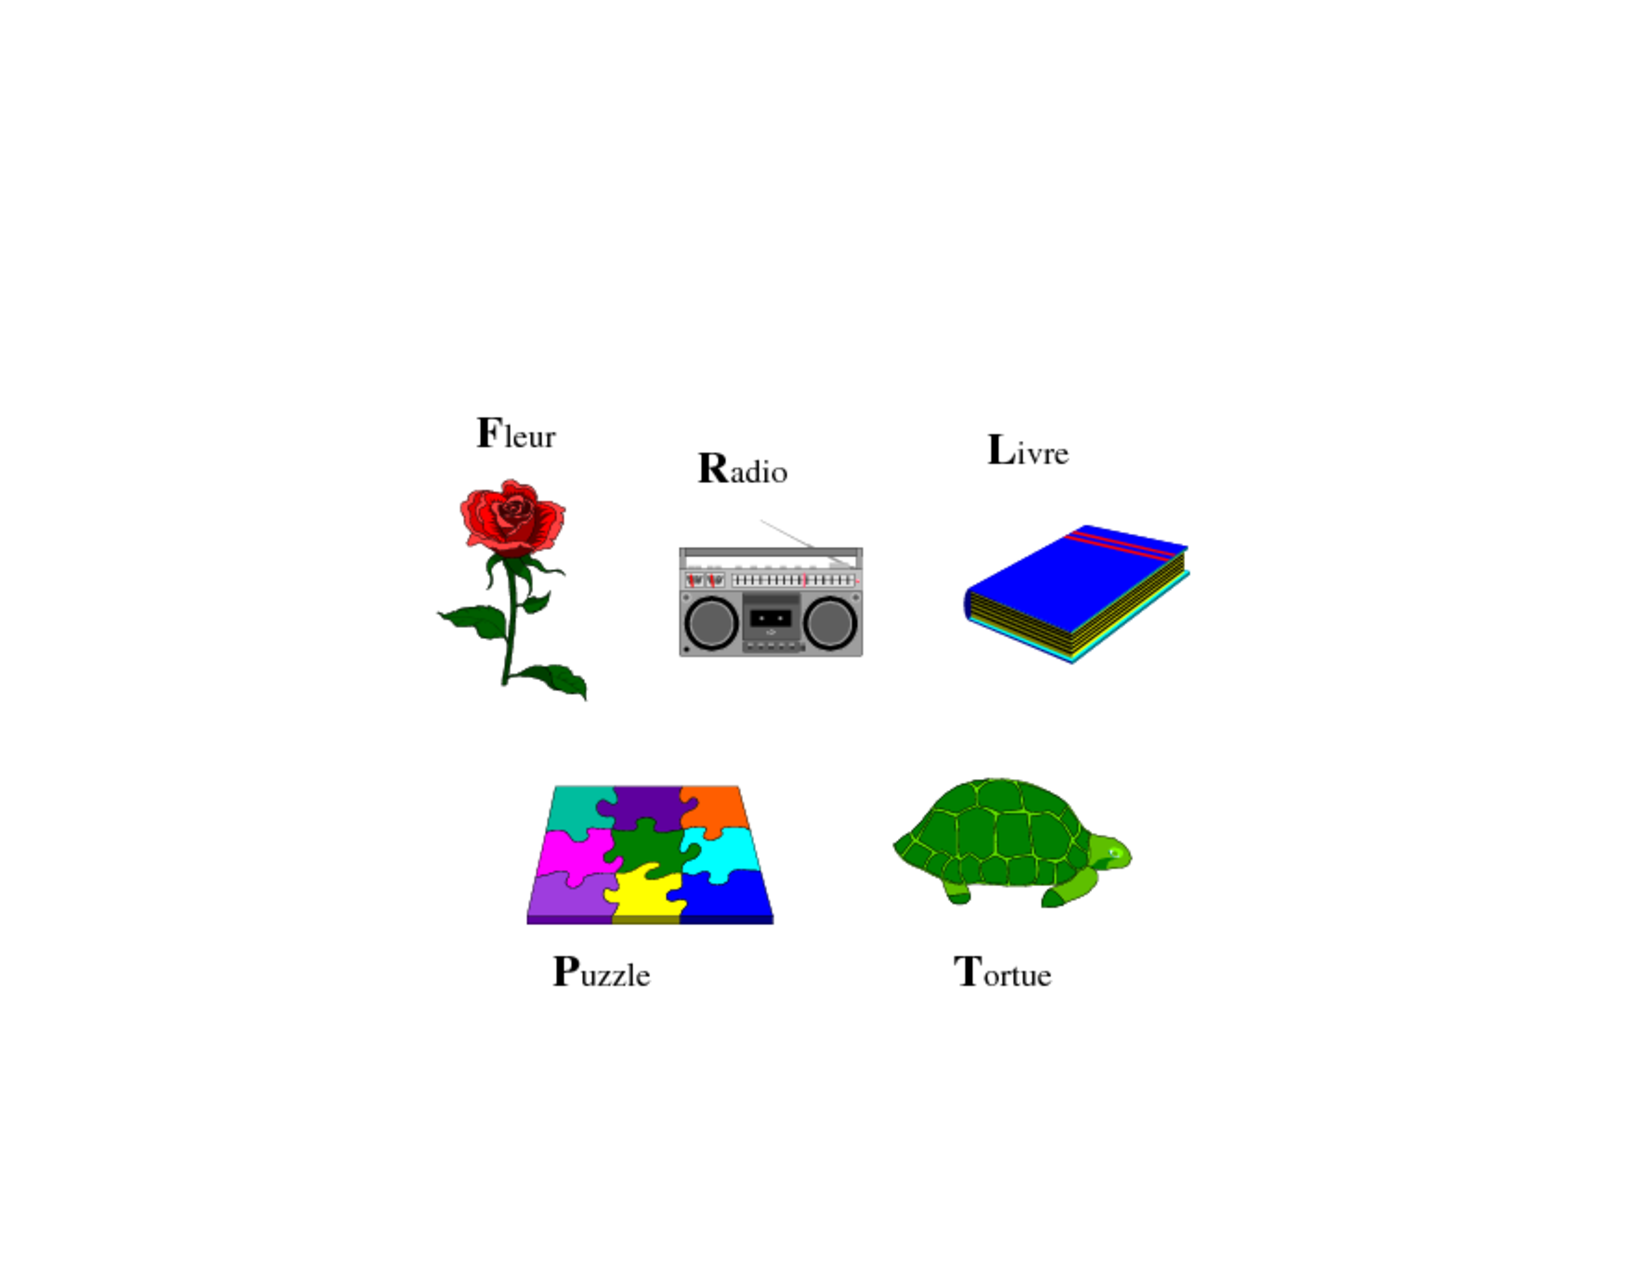
\includegraphics[width=0.4\textwidth,height=0.35\textheight]{gifts.pdf}
\end{figure}

\begin{figure}[h!]
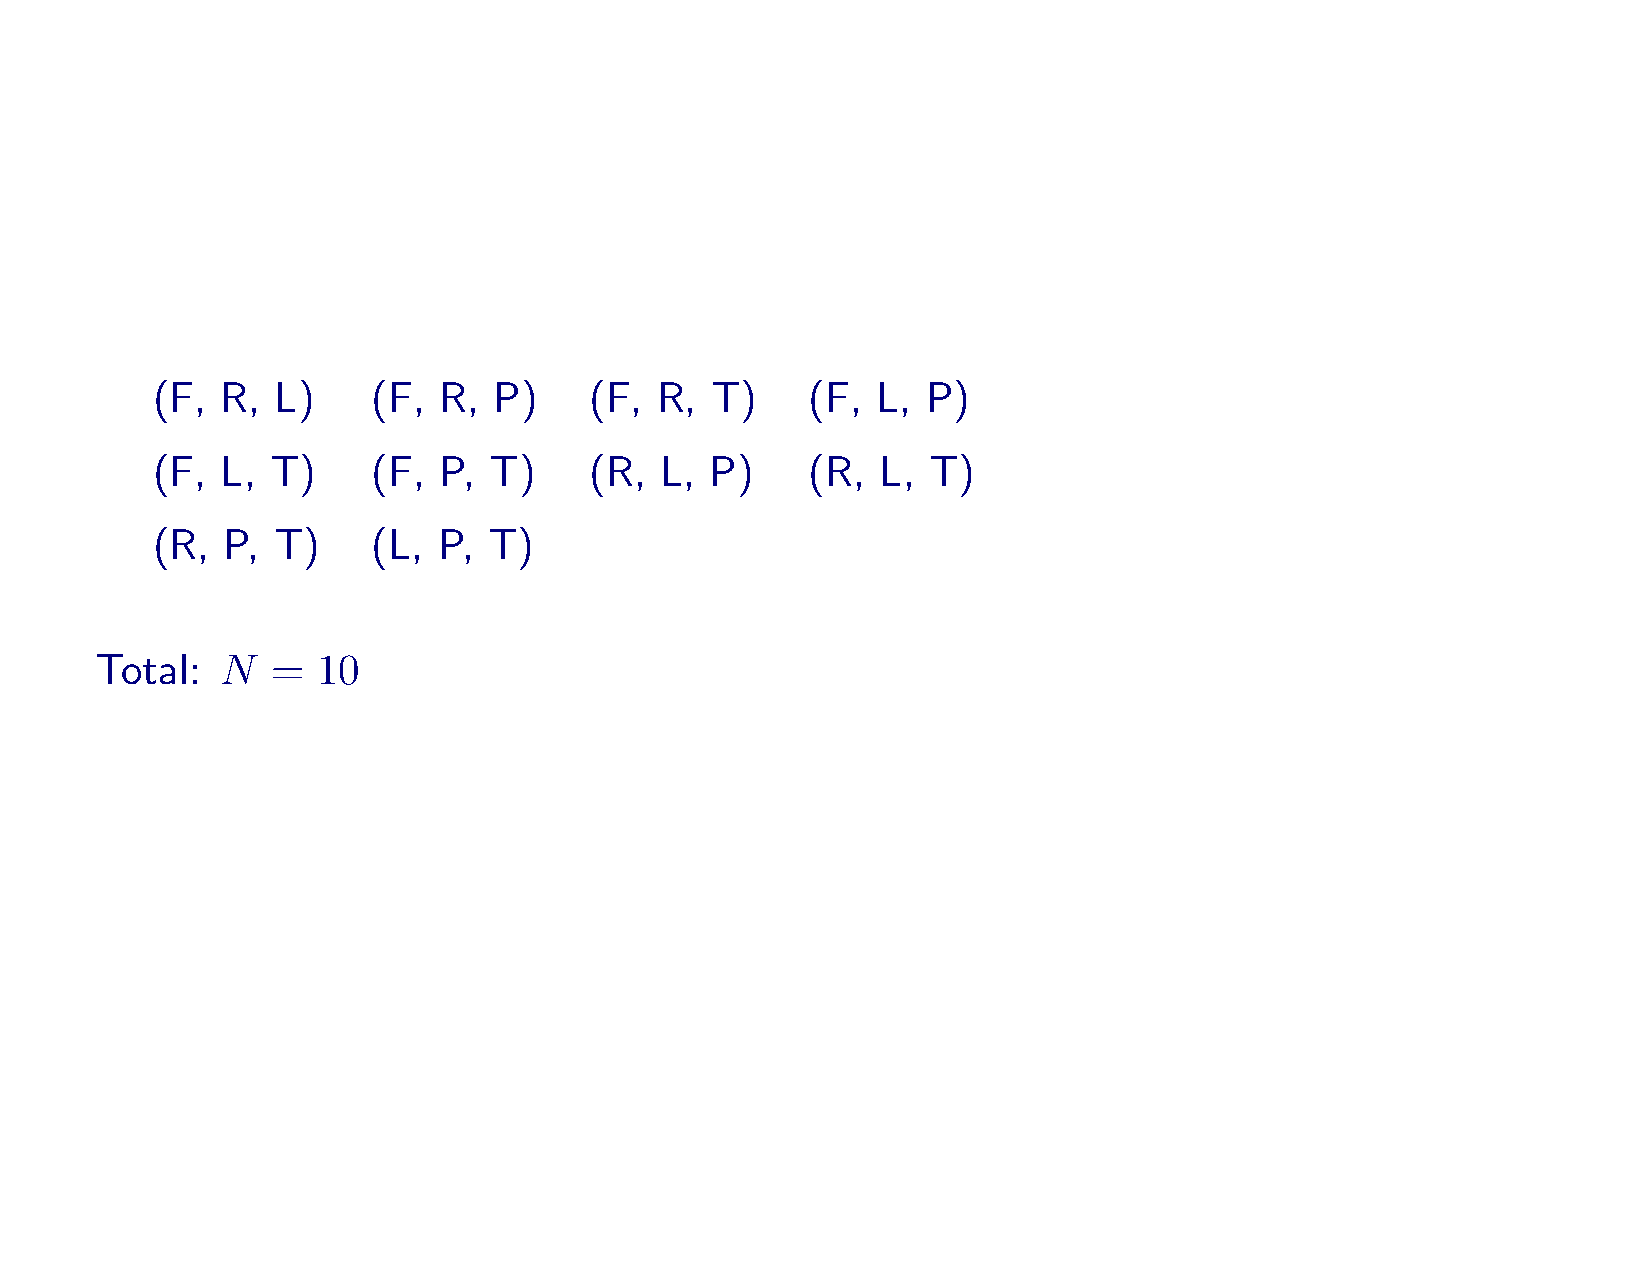
\includegraphics[width=0.5\textwidth,height=0.2\textheight]{outcomes.pdf}
\end{figure}
\end{example}

\end{frame}

%\begin{frame}
%\frametitle{Some mathematical formulas (cont'd)}
%
%\begin{example}[cont'd]
%
%%How many ways can we select $3$ presents (order does not matter) among the $5$ available presents (see figure below)?
%
%\begin{figure}[h!]
%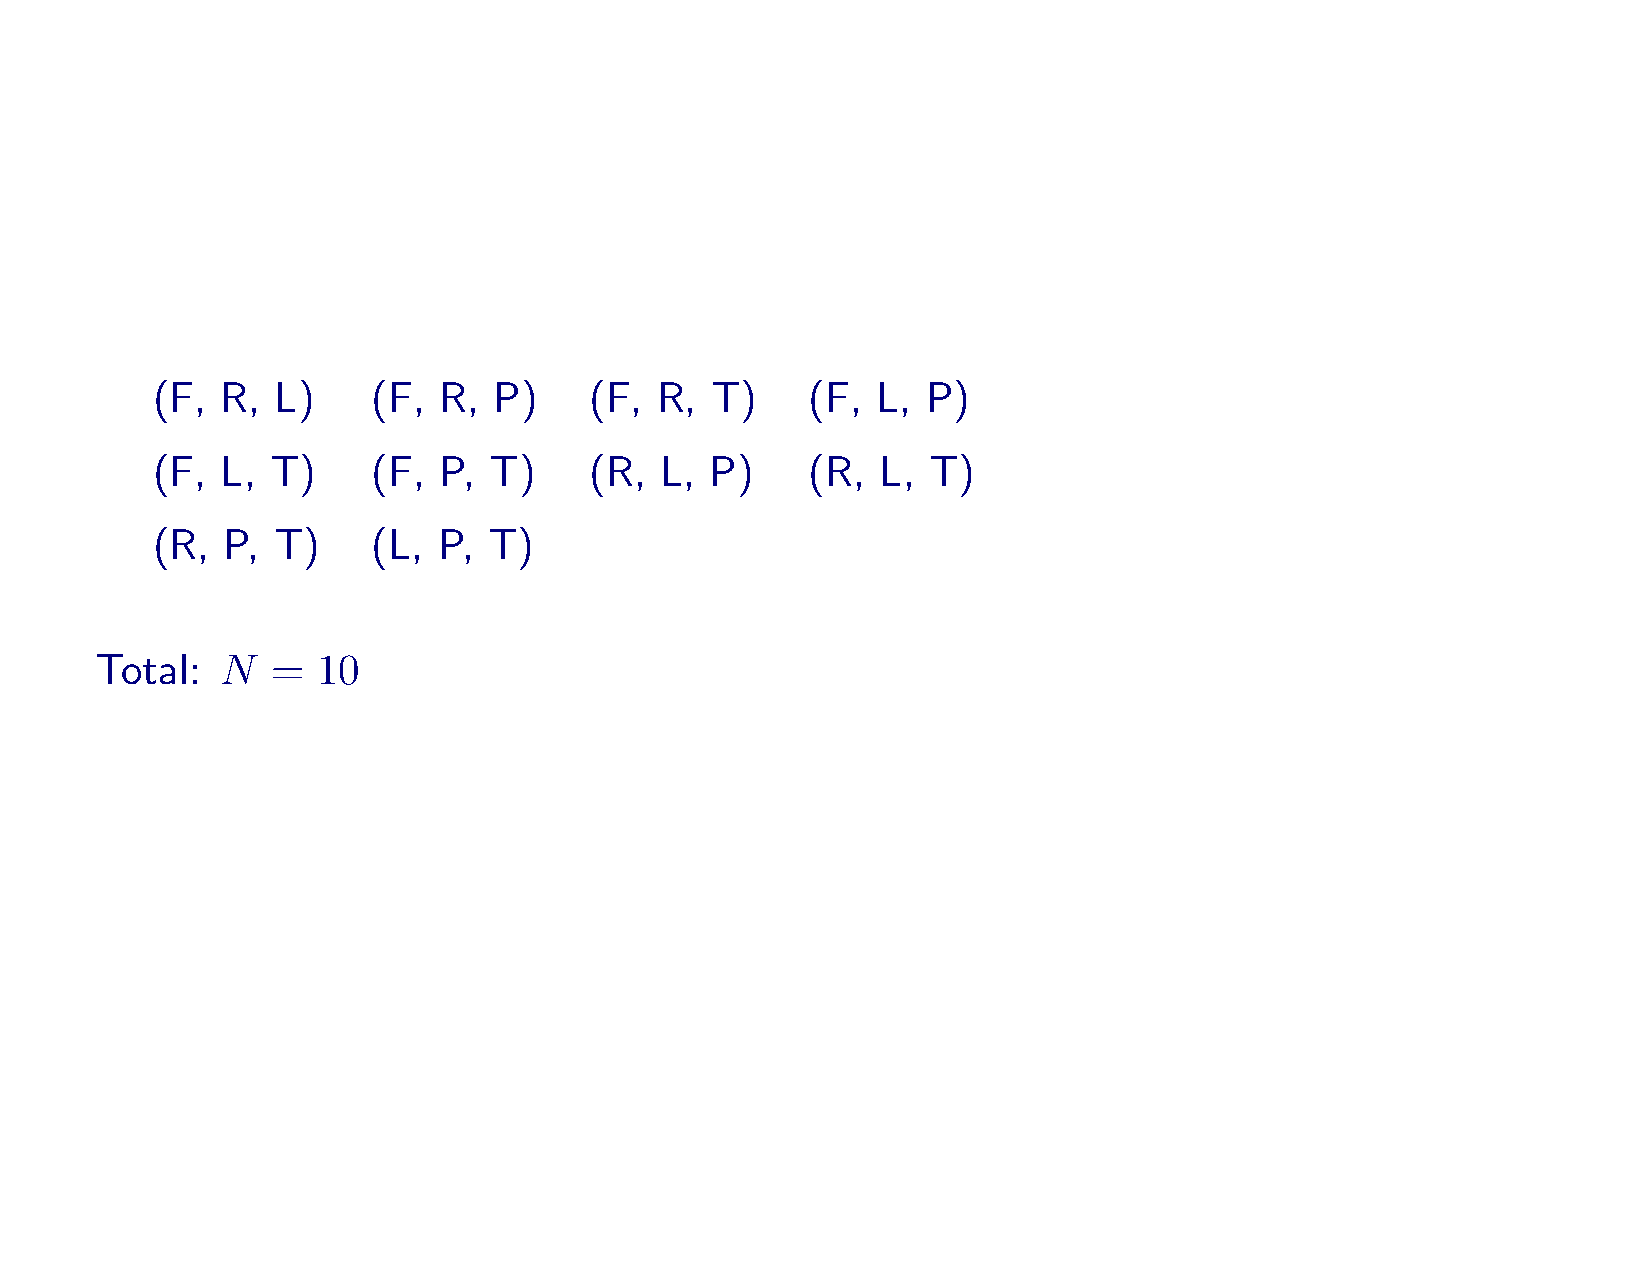
\includegraphics[width=0.6\textwidth,height=0.3\textheight]{outcomes.pdf}
%\end{figure}
%\end{example}
%
%\end{frame}

\begin{frame}
\frametitle{Some mathematical formulas (cont'd)}

\begin{example}[cont'd by Explanation]
\begin{itemize}
\item[1] $5!$ gives you the total $\#$ of possible choices when you can select 5 presents
(so-called ``permutations'', see next slides);
\item[2] If you're going
to select $3$ presents from the list, then you have $(5-3)$ presents that you're not going to select.
Therefore, you need to divide out the $(5-3)!$ different ways you can order the presents
you are not going to select from the $5!$ possible choices of all presents.
In other words you have $5! / (5-3) !$ ways to select and order the 3 presents;
\item[3] Finally, remember you don't care about the order in which you select the $3$ presents. So,
in how many ways can you select $3$ presents from the $n$ available ones? The problem is the same as in [1] above
except that now you don't care about the order of the $3$ presents, and therefore you
also need to divide out the $3!$ different ways you can order the presents.
\end{itemize}
\end{example}

\end{frame}

\begin{frame}
\frametitle{Some mathematical formulas (cont'd)}

\begin{example}[cont'd by Explanation]
... so, in formula, you have $$\frac{5!/(5-3)!}{3!}$$ ways to select the $3$ presents:
$$
\frac{5!/(5-3)!}{3!}= \frac{5!}{3!2!} = \binom 5 3 = C_5^3.
$$
This gives you the total $\#$ of possible ways to select the $3$ presents when the order does not matter.
\end{example}

As a recommendation, redo the exercise assuming you can select 2 presents from 3 available presents
(like for instance F,L,R)...


\end{frame}

\begin{frame}
\frametitle{Some mathematical formulas (cont'd)}

\begin{remark}
\textbf{Permutations:} How many different ways can we combine $n$ objects?
\begin{itemize}
\item In the 1st place: $n$ possibilities
\item In the 2nd place: $(n-1)$ possibilities
\item ...
\item Finally, $1$ possibility
\end{itemize}

Thus, in total we have
$
n\cdot(n-1)\cdot(n-2)\cdot...\cdot1 = n !
$
\end{remark}
\begin{example}
How many ways can Aline, Brigitte and Carmen seat on 3 spots, from left to right? Possible outcomes:
$$
(A, B, C), (A, C, B), (B, A, C), (B, C, A), (C, A, B), (C, B, A)
$$

Total $\#$ of permutations: $N = 6 = 3 \cdot 2 \cdot 1 = 3!$
\end{example}
\end{frame}


\begin{frame}
\frametitle{Some mathematical formulas (cont'd)}

\begin{remark} [cont'd]
\textbf{Combinations:} How many ways can we select $k$ objects among $n$?
To answer this question, we proceed as follows:

\begin{enumerate}
\item How many ways can we combine $k$ objects among $n$?
\begin{itemize}
\item In the 1st place: $n$
\item In the 2nd place: $(n-1)$
\item ....
\item In the $k$-th place: $(n-k+1)$
\end{itemize}

\item We have $k!$ ways to permute the $k$ objects that we selected
\item The number of possibilities (without considering the order) is:
$$
\frac{n!/(n-k)!}{k!} = \frac{n!}{k!(n-k)!} \color{gray}{=C^{k}_n}\color{black}
$$

\end{enumerate}
\end{remark}

\end{frame}

\begin{frame}
\frametitle{Some mathematical formulas (cont'd)}

\begin{remark} [cont'd]

For the Problem Set $2$, you will have to make use of $C^{k}_n$ in Ex2-Ex3-Ex5. Indeed,
to compute the probability for an event $E$, will have to make use of the formula

\begin{equation} \label{Eq: PE}
P(E)=\dfrac{\text{number of cases in E}}{\text{number of possible cases}}.
\end{equation}

This is a first intuitive definition of probability, which we will justify in the next lecture; see Lecture 1, slide 28. For the time being, let us say that the combinatorial calculus will be needed to express both the quantities (numerator
and denominator) in (\ref{Eq: PE}).



\end{remark}

\end{frame}


\begin{frame}
\frametitle{Some mathematical formulas (cont'd)}

Finally, the following \textbf{limits} will be crucial in many tasks:
\begin{itemize}
\item
\bea
\lim_{n \to \infty} \sum_{i=1}^n x_i = \sum_{i=1 }^\infty x_i \nonumber
\eea
\item
\bea
%\lim_{x \to 0} \left(1+x\right)^{\frac{1}{x}} = \lim_{x \to \infty} \left(1+\frac{1}{x}\right)^{x} = e \nonumber
e^x = \lim_{n \rightarrow \infty} \left(1 + \frac{x}{n}\right)^n \nonumber
\eea
\item for $\alpha >0$
\bea
\lim_{x \to \infty} {\alpha e^{-\alpha x}} = 0 \nonumber
\eea
\item
\bea
e^x = \sum_{i = 0}^{\infty} {x^i \over i!} = 1 + x + {x^2 \over 2!} + {x^3 \over 3!} + {x^4 \over 4!} + \cdots \nonumber
\eea

\end{itemize}
\end{frame}



\end{document}

